% 第 4 章 Using Design Planning Tools
\bichapter{使用设计规划工具}{Using Design Planning Tools}
\label{chap:gui-dp}

IC Compiler II GUI 提供支持设计规划（design planning）中各项任务的工具。假设通道拥塞（What-if Channel Congestion）工具支持交互式假设分析（what-if analysis），用来找出拥塞的全局布线通道。层次探索（Hierarchy Exploration）工具支持与模块边界（module boundary）相关的若干任务。

下列主题说明 GUI 所支持的设计规划任务：
\begin{itemize}
  \item 层次浏览器
  \item 基于名称的层次浏览器
  \item 假设通道拥塞
  \item 层次探索
  \item 拓扑管脚约束
  \item 使用管脚约束
  \item 执行拓扑互连规划
\end{itemize}

\section{层次浏览器}
\subsection*{Hierarchy Browser}

本工具提供用于探索设计层次的工具，以便确定要把哪些逻辑层次单元提交（commit）为物理层次块。GUI 中的层次浏览器（Hierarchy Browser）显示设计层次，并提供每个层次单元的其他信息。

用 Hierarchy Browser 探索设计层次：
\begin{enumerate}
  \item 在 GUI 中选择 \textbf{View > Hierarchy Browser}。
  \item 单击层次单元旁的 [+] 符号，展开或折叠层次。
  \item 单击列标题，重排显示。
  \item 单击块名，对该块执行其他操作。
\end{enumerate}

Hierarchy Browser 中显示的层次示例如图~\ref{fig:gui-56} 所示。

\begin{figure}[htbp]
\centering
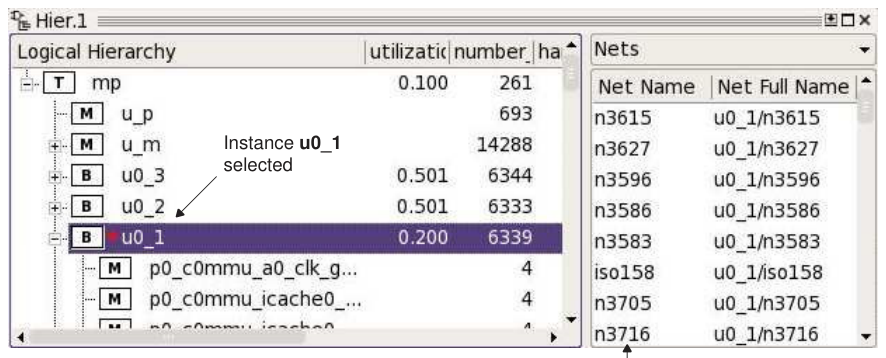
\includegraphics[width=0.92\textwidth]{gui-fig-056.png}
\caption{层次浏览器}
\label{fig:gui-56}
\end{figure}

在 Hierarchy Tree 视图中使用上下文菜单时，在逻辑层次上右键单击即可打开菜单，并执行下列操作：
\begin{itemize}
  \item 选择 \textbf{Partitioning > Create Module Boundary}，为指定层次级别创建模块边界。
  \item 选择 \textbf{Partitioning > Create Bound}，创建模块边界，并在版图窗口中启动 Create Bound 工具。在版图窗口中画出约束（bound），以完成该任务。
  \item 选择 \textbf{Partitioning > Copy Macro Relative Placement}，把硬宏（hard macro）的相对布局复制到所选模块。
  \item 选择 \textbf{Color by Hierarchy > Set Selected Color}，再从菜单中选择一种颜色，改为指定颜色。
  \item 选择 Commit Block，把逻辑层次单元提交为物理层次块。
  \item 选择 Clear Selection，取消层次中全部已选对象的选择。
  \item 选择 Select Related Objects，再从列表中选择一项，以选择与该对象关联的连接、宏、安全核规则（safety core rule）、安全核组（safety core group）等。
\end{itemize}

也可以从下列位置之一查看相关对象：
\begin{itemize}
  \item 版图视图（Layout view）
  \item Select 菜单：
  \begin{itemize}
    \item \textbf{Select > By Name Toolbar}，或
    \item \textbf{Select > By Name}，或
    \item \textbf{Select > Related Objects}，或
  \end{itemize}
  \item 上下文相关菜单（右键单击对象，再选择 \textbf{Select Related Objects}）
\end{itemize}

例如，选中一条拓扑边（topology edge）或一个拓扑规划（topology plan）时，上下文菜单会随之显示。

使用 Selection List 面板、Properties 面板或 Queries 面板，查看所选对象的更多细节。
\begin{itemize}
  \item 选择 Properties，打开对话框，显示所选逻辑层次的属性。
  \item 选择 Expand Tree，显示所选逻辑层次的子层次。
  \item 选择 Copy Text，复制所选单元的名称。复制的文本同时进入复制缓冲区（copy buffer）和剪贴板。
\end{itemize}

可从 Hierarchy Tree 视图和 Child List 视图使用该功能。
\begin{itemize}
  \item 选择 Find Copied Cell Text，搜索已复制的单元，并在 Hierarchy Tree 视图中选中它。
\end{itemize}

只有用 Copy Text 功能复制过单元名之后，才能使用该功能。
\begin{itemize}
  \item 选择 \textbf{Set Hierarchy Root > Set Root to Current Selected Cell}，更改层次树的根，并对所选对象执行操作。
\end{itemize}

在列标题上右键单击可打开上下文菜单。可以在 Child List 视图的上下文菜单中执行下列操作。

\begin{noteBox}
上下文菜单只对特定标题可用。
\end{noteBox}

\begin{itemize}
  \item 选择 Compress Bus Objects (User Table)，把带总线记法（bus notation）的对象导出到用户表（User Table），并把全部公共对象名压缩为单个总线对象（bused object）。
  \item 使用已压缩 User Table 上下文菜单中的过滤选项，查看总线对象、总线内容，或返回完整的总线表。
\end{itemize}

可以在 TreeMap 视图中执行下列操作：

在 Hier Std Color 对话框上选择 Outliers，高亮设计中落在指定最小值与最大值范围之外的那些单元。

\subsection{在层次浏览器中过滤信息}
\subsubsection*{Filtering Information in the Hierarchy Browser}
\label{sec:gui-dp-filter}

层次浏览器支持列过滤，并用过滤框过滤表中的信息。要显示过滤表达式框，执行下列操作之一：
\begin{itemize}
  \item 按正斜杠键（/），或
  \item 在列标题上右键单击，打开过滤选项。
\end{itemize}

\begin{figure}[htbp]
\centering
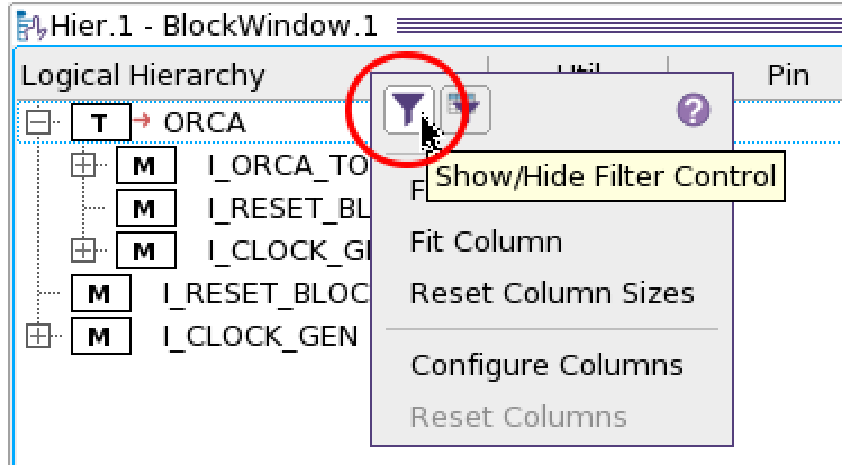
\includegraphics[width=0.92\textwidth]{gui-fig-057.png}
\caption{启用过滤}
\label{fig:gui-57}
\end{figure}

在表达式框中输入表达式，只显示与该表达式匹配的条目。

\begin{figure}[htbp]
\centering
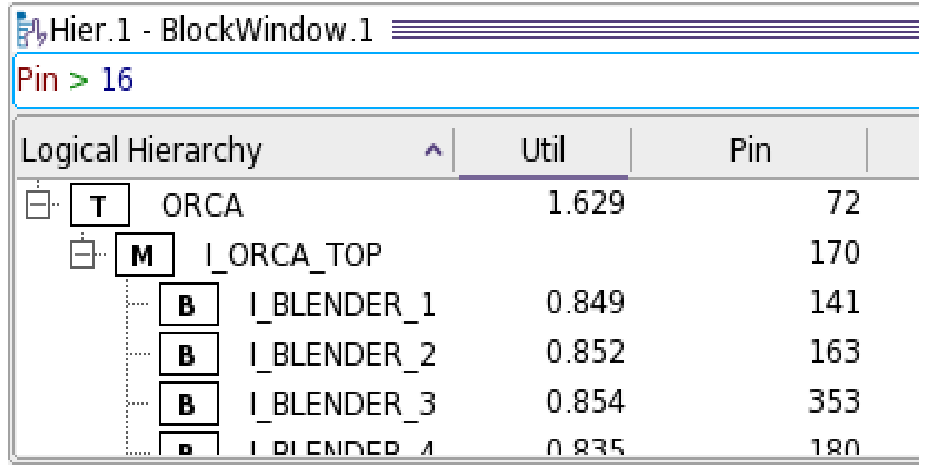
\includegraphics[width=0.92\textwidth]{gui-fig-058.png}
\caption{过滤表达式}
\label{fig:gui-58}
\end{figure}

要启用列过滤，单击过滤框右侧的 Show/Hide Column filter 控件按钮。也可以在列标题上单击鼠标右键，再单击上下文菜单中的按钮，如图~\ref{fig:gui-59} 所示。

\begin{figure}[htbp]
\centering
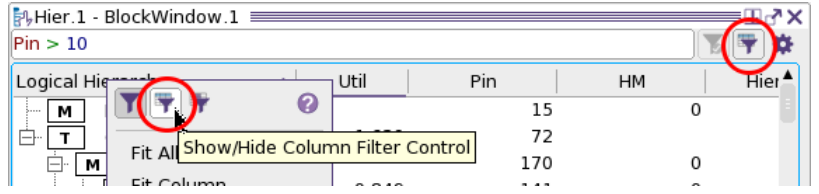
\includegraphics[width=0.92\textwidth]{gui-fig-059.png}
\caption{启用列过滤}
\label{fig:gui-59}
\end{figure}

要查看 Column Filter 菜单，单击漏斗图标。用菜单中的选项按升序或降序排列该列、创建过滤条件，或通过选择列中的特定值来过滤该列。过滤菜单如图~\ref{fig:gui-60} 所示。

\begin{figure}[htbp]
\centering
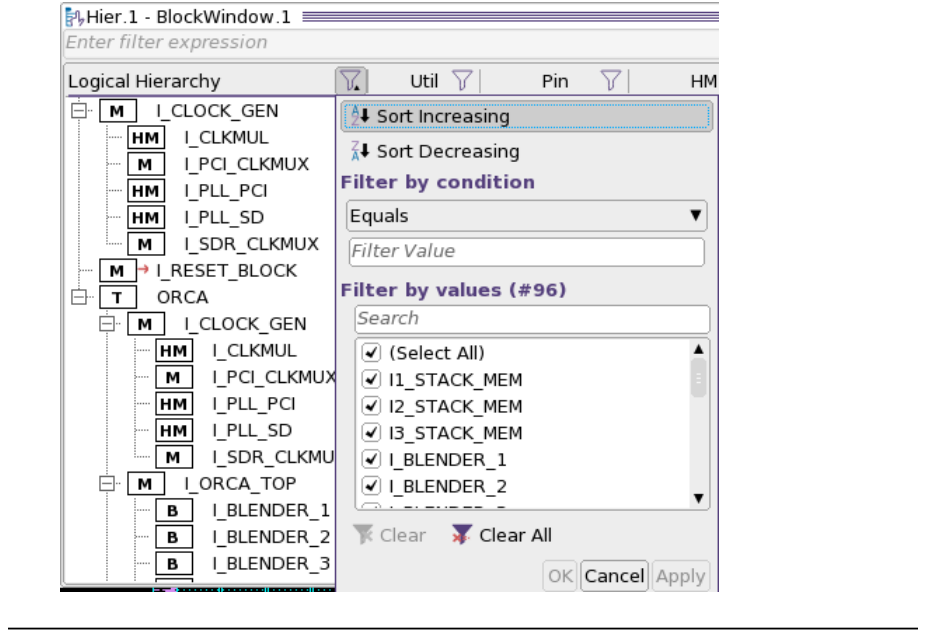
\includegraphics[width=0.92\textwidth]{gui-fig-060.png}
\caption{列过滤菜单}
\label{fig:gui-60}
\end{figure}

\section{基于名称的层次浏览器}
\subsection*{Name Based Hierarchy Browser}

对于扁平设计（flat design），本工具提供基于名称的层次浏览器（Name Based Hierarchy Browser），用来显示设计中的隐含层次（implicit hierarchy），并允许对层次执行操作。

要启动 Name Based Hierarchy Browser，选择 \textbf{View > Name Based Hierarchy Browser}。工具按图~\ref{fig:gui-61} 所示显示该浏览器。若设计含有层次，该选择被禁用，不能使用此功能。

\begin{figure}[htbp]
\centering
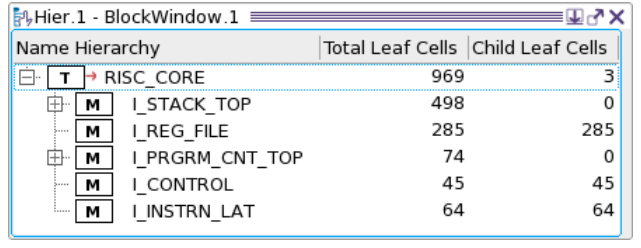
\includegraphics[width=0.92\textwidth]{gui-fig-061.png}
\caption{基于名称的层次浏览器}
\label{fig:gui-61}
\end{figure}

工具根据应用选项 \appopt{gui.name\_based\_hier\_delimiter} 的设置提取层次。默认值为「/」。可以用 \cmd{ungroup\_cells -all -flatten} 命令把设计转换为扁平设计。

与 Hierarchy Browser 类似，可以用上下文菜单执行不同操作；在层次上右键单击即可显示上下文菜单：
\begin{itemize}
  \item 选择 Set Colors On Top Hierarchies，为每个顶层层次指定一种颜色
  \item 选择 Clear All Hierarchy Colors，去掉层次上的全部颜色
  \item 选择 Set Selected Hierarchy Color 并选择一种颜色，为所选层次指定颜色
  \item 选择 Clear Selected Hierarchy Color，去掉当前所选层次的颜色
  \item 选择 Show Child List，拆分对话框并显示所选层次中的单元列表
  \item 选择 Expand All Hierarchy Trees 并选择层数，显示全部顶层层次的子层次
  \item 选择 Expand Selected Hierarchy Trees 并选择层数，显示所选层次的子层次
  \item 选择 Copy Hierarchy Path，把当前层次的实例路径复制到剪贴板
\end{itemize}

\begin{seeAlsoBox}
表中结果的过滤方法，见第~\ref{sec:gui-dp-filter}~节。
\end{seeAlsoBox}

\section{假设通道拥塞}
\subsection*{What-if Channel Congestion}

IC Compiler II 工具支持交互式假设分析，用来找出拥塞的全局布线（global routing）通道（channel）。要在版图窗口中打开 What-if Channel Congestion 图模式，在 Task Assistant 的 Design Planning 区中选择 What-if Channel Congestion，或选择 \textbf{View > Map > What-if Channel Congestion}。What-if Channel Congestion 图模式出现在版图窗口右侧，如图~\ref{fig:gui-62} 所示。

\begin{figure}[htbp]
\centering
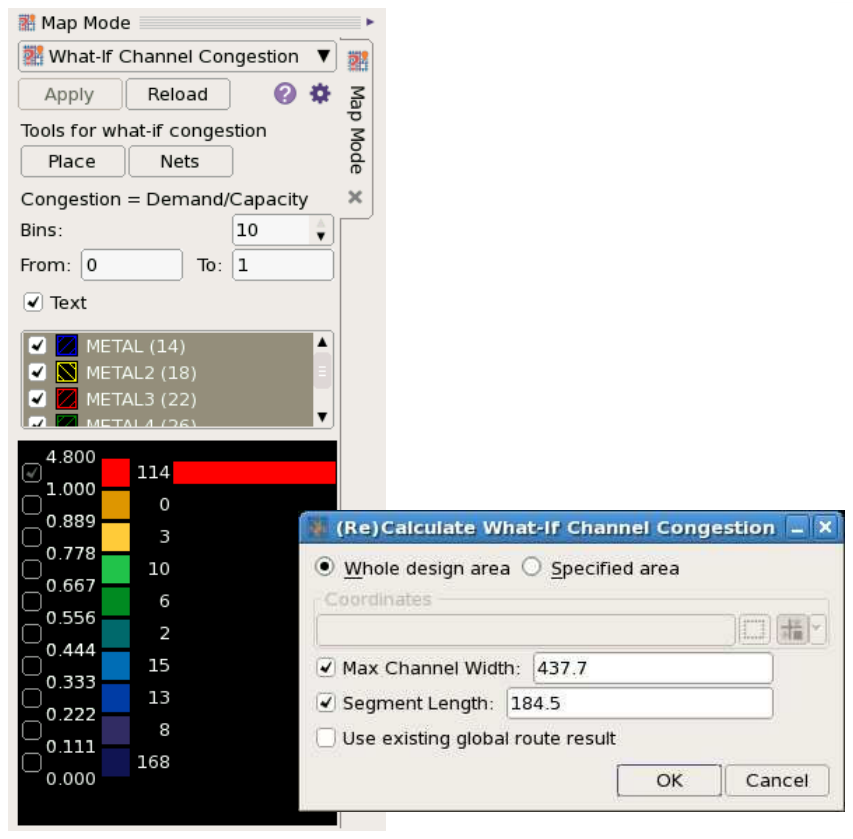
\includegraphics[width=0.92\textwidth]{gui-fig-062.png}
\caption{假设通道拥塞图模式与 Reload 对话框}
\label{fig:gui-62}
\end{figure}

\subsection{为假设通道拥塞执行全局布线}
\subsubsection*{Performing Global Routing for What-if Channel Congestion}

开始假设拥塞分析：
\begin{enumerate}
  \item 单击 Reload 按钮，打开 Calculate What-If Channel Congestion Map Data 对话框。
  \item 选择 Whole design area 或 Specified area，确定要评估的设计区域。
  \item （可选）更改 Max Channel Width 框中的值，设置要显示的最大通道尺寸；按通道宽度过滤的更多说明，见第~\ref{sec:gui-dp-chan-min}~节。
  \item （可选）更改 Segment Length；关于段长度的更多说明，见第~\ref{sec:gui-dp-chan-seg}~节。
  \item （可选）选择 Use existing global route result，使用来自 \cmd{route\_global -congestion\_map\_only true} 命令的已有布线信息。
\end{enumerate}

可以用 \cmd{remove\_routes -global\_route} 命令从设计中删除全局布线。
\begin{enumerate}
  \setcounter{enumi}{5}
  \item 单击 OK，创建拥塞图（congestion map）。
\end{enumerate}

\subsection{查看拥塞信息}
\subsubsection*{Viewing Congestion Information}

全局布线完成后，工具高亮设计中每条拥塞通道。要显示该通道的更多信息，把指针移到通道上并查看信息提示（infotip）。信息提示显示该通道以及通道内沿优选布线方向（preferred routing direction）每一层金属的需求（demand）与容量（capacity）。图~\ref{fig:gui-63} 是一条拥塞通道的信息提示。

\begin{figure}[htbp]
\centering
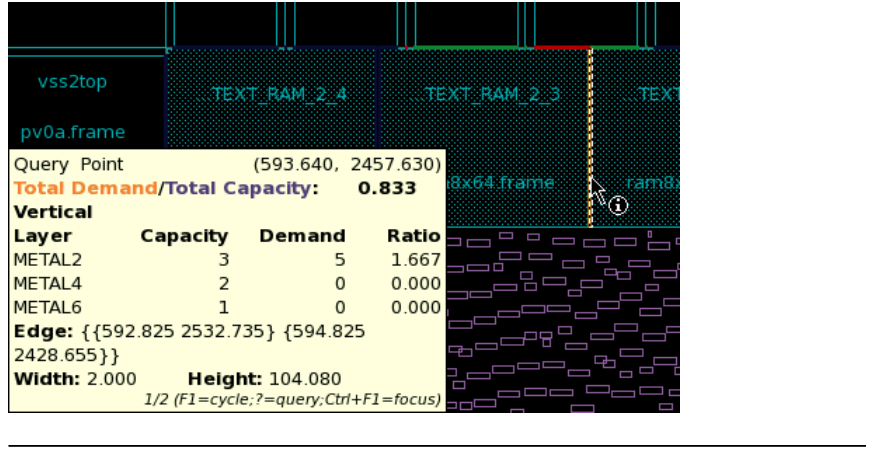
\includegraphics[width=0.92\textwidth]{gui-fig-063.png}
\caption{假设通道拥塞信息提示}
\label{fig:gui-63}
\end{figure}

\subsection{按最小通道尺寸过滤}
\subsubsection*{Filtering by Minimum Channel Dimension}
\label{sec:gui-dp-chan-min}

要只显示设计中的窄通道，单击 Reload 按钮，在 Max channel width 框中输入通道宽度值，再单击 OK。工具更新显示，并隐藏最小尺寸（高度或宽度）大于指定最大通道宽度值的通道，如图~\ref{fig:gui-64} 所示。

\begin{figure}[htbp]
\centering
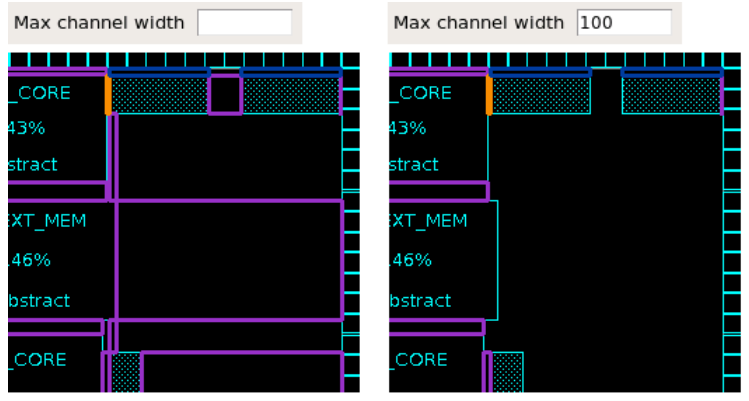
\includegraphics[width=0.92\textwidth]{gui-fig-064.png}
\caption{按最小通道尺寸过滤}
\label{fig:gui-64}
\end{figure}

\subsection{显示通道段}
\subsubsection*{Displaying Channel Segments}
\label{sec:gui-dp-chan-seg}

要做更细致的分析并把通道划分成更小的段（segment），在 Segment length 框中输入一个值。工具细分每条通道，并创建指定长度的段，如图~\ref{fig:gui-65} 所示。沿通道移动指针，在信息提示中查看每个通道段的详细拥塞信息。

\begin{figure}[htbp]
\centering
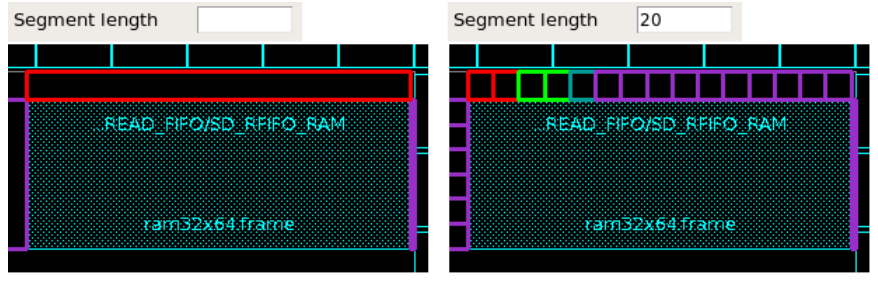
\includegraphics[width=0.92\textwidth]{gui-fig-065.png}
\caption{带分段的通道}
\label{fig:gui-65}
\end{figure}

请注意，段尺寸可能与指定值并不完全一致。某些情况下，工具会增大或缩小线段，以形成尺寸一致的段。

\subsection{指定分析区域}
\subsubsection*{Specifying the Region for Analysis}

默认情况下，工具为整个设计生成假设拥塞图。可以指定一个区域来限制分析，从而加快拥塞分析。单击 Region 框右侧的按钮，在版图窗口中画一个矩形，再单击 Apply，把分析限制在所画区域。也可以在 Region 框中指定包围盒（bounding box）的坐标，再单击 OK，只分析指定区域。

\subsection{缩放拥塞颜色映射}
\subsubsection*{Scaling the Congestion Color Mapping}

工具根据通道中所需布线数与可用布线数之比，为每条通道着色。默认情况下，比值超过 1.0（所需布线数超过可用布线数）的通道着红色，比值小于 0.2 的通道着紫色。

要更改通道的着色方式，在 From: 与 To: 框中输入值，再单击 Apply。工具重新显示拥塞图，并按这些值给通道着色。

\subsection{修正拥塞问题}
\subsubsection*{Correcting Congestion Problems}

要用 What-if Channel Congestion 分析以交互方式减轻布线拥塞，执行下列操作：
\begin{enumerate}
  \item 选择与拥塞区域邻接的硬宏
  \item 按 M，或从工具栏选择 Move 工具
  \item 用鼠标移动硬宏，在拥塞区域形成更宽的通道
\end{enumerate}

也可以按 Tab 键，在 Move 工具栏的 Delta 框中输入 x 与 y 偏移，再按 Enter。工具按指定距离移动硬宏。把硬宏移到新位置后，工具根据更新后的布局重新显示拥塞图。

重复这些步骤，直到对拥塞图和布局满意。修复前后的版图如图~\ref{fig:gui-66} 所示。

\begin{figure}[htbp]
\centering
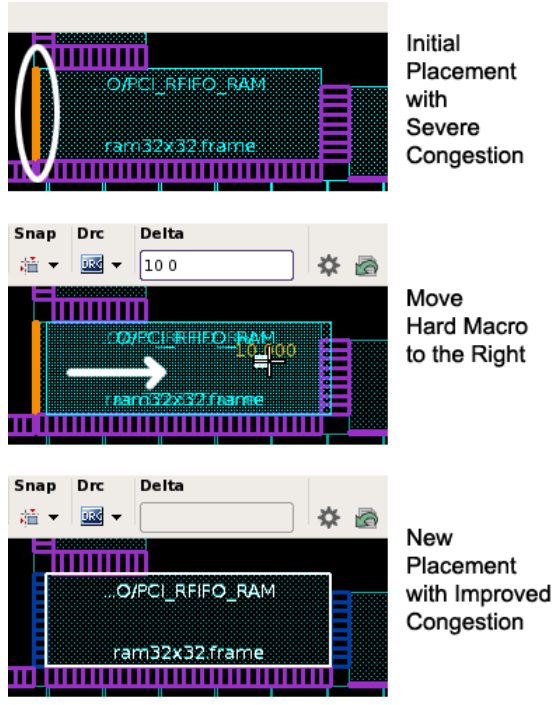
\includegraphics[width=0.92\textwidth]{gui-fig-066.png}
\caption{假设拥塞修复}
\label{fig:gui-66}
\end{figure}

\subsection{更新布局}
\subsubsection*{Updating the Placement}

调整通道宽度后，单击 Place 按钮更新单元布局。工具运行 \cmd{create\_placement -floorplan -effort medium} 命令更新布局，同时使单元保持在原先位置附近。

\subsection{显示通道中的线网}
\subsubsection*{Showing Nets in a Channel}

要显示占用某条特定通道的线网连接，单击 Nets 按钮，再在通道中单击。工具显示穿过该通道的线网，以及它们在通道外的路径。图~\ref{fig:gui-67} 是显示穿过通道的线网之前与之后的版图。要清除显示，在通道外任意位置单击。

\begin{figure}[htbp]
\centering
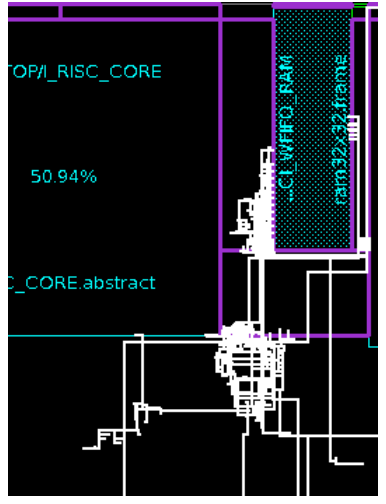
\includegraphics[width=0.92\textwidth]{gui-fig-067.png}
\caption{显示通道中的线网}
\label{fig:gui-67}
\end{figure}

\subsection{去掉拥塞图}
\subsubsection*{Removing the Congestion Map}

要从版图中去掉 What-if Channel Congestion 图，关闭 What-If Channel Congestion 图模式面板。

\section{层次探索}
\subsection*{Hierarchy Exploration}

在 IC Compiler II 工具中，模块边界表示逻辑层次中尚未提交的块。利用模块边界，可以快速评估顶层块在给定利用率（utilization）下大约需要的块尺寸，并在平面规划（floorplan）内排列模块边界，以便粗略估计块的布局。

要在版图窗口中打开 Hierarchy Exploration 面板，在 Task Assistant 的 Design Planning 区中选择 Hierarchy Exploration，或在 GUI 中选择 \textbf{View > Assistants > Hierarchy Exploration}。Hierarchy Exploration 面板出现在版图窗口右侧。

\subsection{创建模块边界}
\subsubsection*{Creating Module Boundaries}

要创建模块边界，单击 Hierarchy Exploration 面板中的 Initialize 按钮。工具为顶层模块插入模块边界，如图~\ref{fig:gui-68} 所示。

\begin{figure}[htbp]
\centering
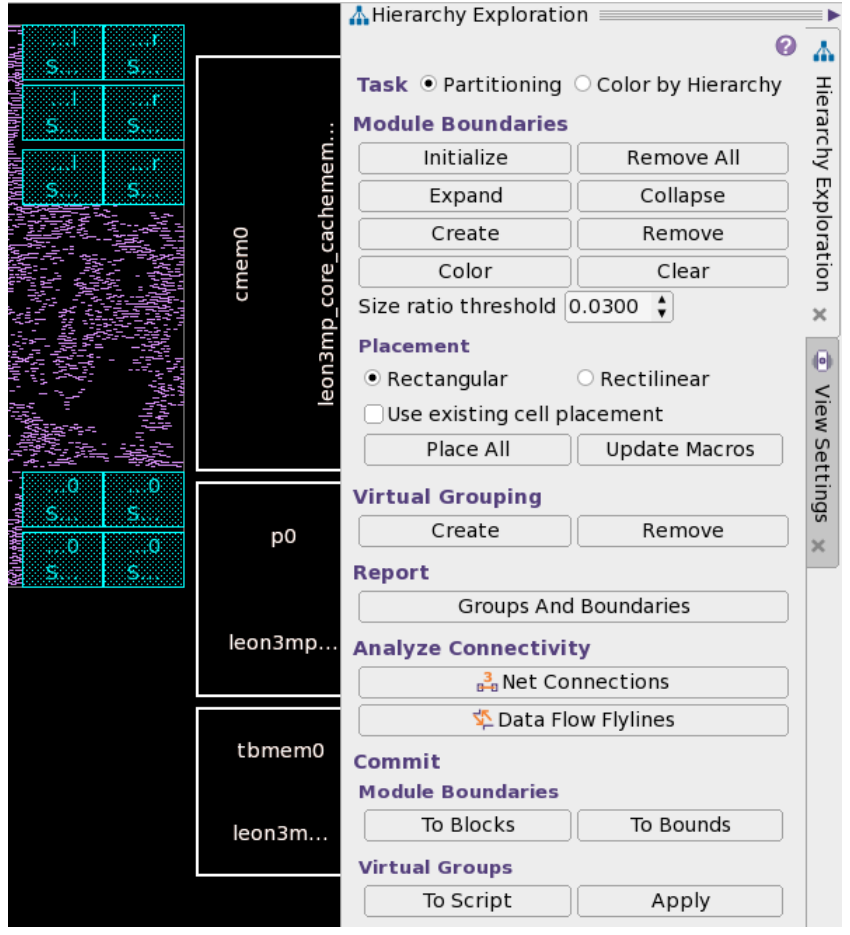
\includegraphics[width=0.92\textwidth]{gui-fig-068.png}
\caption{初始化后的模块边界}
\label{fig:gui-68}
\end{figure}

可以用 \cmd{explore\_logic\_hierarchy -create\_module\_boundary} 命令执行同一操作。

也可以用 GUI 中的 Hierarchy Browser 为所选模块创建模块边界。用 Hierarchy Browser 创建模块边界：
\begin{enumerate}
  \item 选择 \textbf{View > Hierarchy Browser}
  \item 选择一个逻辑层次块
  \item 从上下文菜单选择 Create Module Boundary，或单击 Hierarchy Exploration 面板 Module Boundaries 区中的 Create 按钮
\end{enumerate}

\subsection{展开、折叠与删除模块边界}
\subsubsection*{Expanding, Collapsing, and Removing Module Boundaries}

要把模块边界展开为子模块，选择该模块边界并单击 Expand。要把模块边界折叠进其父模块，选择该模块边界并单击 Collapse。要删除一个或多个模块边界，选择这些模块边界并单击 Remove。要删除全部模块边界，单击 Remove All。

也可以用上下文菜单执行这些操作。
\begin{enumerate}
  \item 选择一个或多个模块边界
  \item 在所选模块边界之一上右键单击，并从上下文菜单选择操作（Expand、Collapse 或 Remove Module Boundary）
\end{enumerate}

\subsection{为模块边界着色}
\subsubsection*{Coloring Module Boundaries}

要为每个模块边界应用互不相同的颜色，单击 Color。再次单击 Color，应用另一种配色方案。要去掉模块边界上的任何着色，单击 Clear。

\subsection{放置模块边界}
\subsubsection*{Placing Module Boundaries}

要把模块边界放入核区域（core area）：
\begin{enumerate}
  \item 选择布局类型：矩形（rectangular）或直角多边形（rectilinear）。两种布局类型的示例见图~\ref{fig:gui-69}
  \item 选择 Use existing cell placement，按已有布局放置模块边界
  \item 单击 Place All，把模块边界放入核区域
\end{enumerate}

\begin{figure}[htbp]
\centering
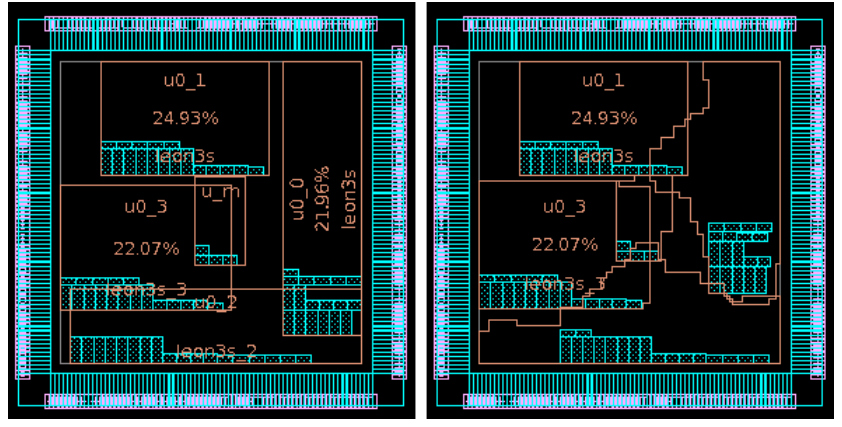
\includegraphics[width=0.92\textwidth]{gui-fig-069.png}
\caption{矩形与直角多边形模块边界布局}
\label{fig:gui-69}
\end{figure}

要把属于某个模块约束的硬宏移入模块边界内部，单击 Update Macros。

\subsection{层次探索与模块颜色}
\subsubsection*{Hierarchy Exploration and Module Color}

Hierarchy Exploration 面板提供工具，为模块边界以及设计边界内与之对应的标准单元和宏添加颜色。工具还会在设计内不同层次周围画出边界。在面板顶部 Task 区中选择 “Color by Hierarchy”，即可使用这些功能。

\begin{figure}[htbp]
\centering
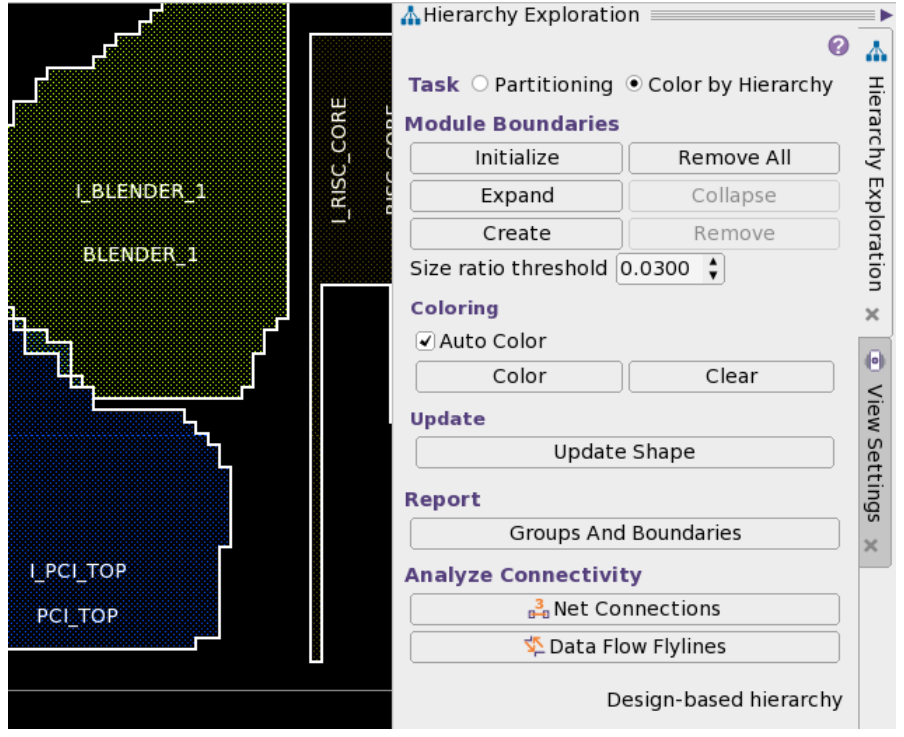
\includegraphics[width=0.92\textwidth]{gui-fig-070.png}
\caption{层次探索中的按层次着色}
\label{fig:gui-70}
\end{figure}

\subsection{在版图中查看层次}
\subsubsection*{Viewing Hierarchies in the Layout}

要在版图中高亮不同层次：
\begin{enumerate}
  \item 从菜单选择 \textbf{View > Assistants > Hierarchy Exploration}。
  \item 在面板的 Task 区中选择 “Color by Hierarchy”。
  \item 在面板的 Module Boundaries 区单击 Initialize，创建模块边界。
\end{enumerate}

工具高亮并选择全部顶层层次。
\begin{enumerate}
  \setcounter{enumi}{3}
  \item （可选）单击 Color 更改模块颜色，单击 Clear 去掉全部模块颜色。
  \item （可选）打开 Hierarchy Browser 并选择一个或多个层次，更改被高亮的层次。
\end{enumerate}

\subsection{假设划分}
\subsubsection*{What-if Partitioning}

假设划分（what-if partitioning）帮助查看不同模块边界之间的关系，并通过创建虚拟组（virtual group）来组织模块边界的层次。在假设划分期间，可以：
\begin{itemize}
  \item 用 Net Connections 或 Data Flow Flylines 工具查看不同模块边界之间的连接关系
  \item 创建包含相互连接的模块边界的虚拟组
  \item 通过放置、合并或删除虚拟组，考察不同的划分策略
  \item 写出模块边界分组，供重新综合（resynthesis）使用
\end{itemize}

要显示模块边界之间的连接关系：
\begin{enumerate}
  \item 单击 Hierarchy Exploration 面板中的 Net Connections 按钮。
  \item 在 Net Connections 面板的 Connectivity Display 区中选择 Selected to Selected。
  \item 单击一个模块边界，再单击一个或多个其他边界，查看它们之间的连接关系。
\end{enumerate}

要创建虚拟组：
\begin{enumerate}
  \item 只选择要合并进新模块组的模块边界或模块组。
  \item 单击 Hierarchy Exploration 面板 Virtual Grouping 区中的 Create 按钮。
  \item （可选）选择某个虚拟组并单击 Remove 按钮，取消该虚拟组的分组。
\end{enumerate}

图~\ref{fig:gui-71} 左侧，两个模块边界被选中，并显示了所选模块的线网连接。这两个模块共享公共线网连接，适合分在一组。右侧是单击 Create 按钮后已分组的模块。可以把指针移到模块组上，在信息提示中显示该组的信息。

\begin{figure}[htbp]
\centering
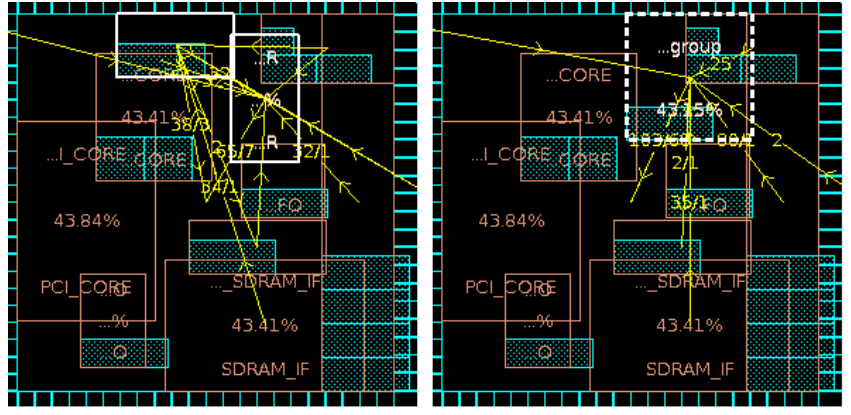
\includegraphics[width=0.92\textwidth]{gui-fig-071.png}
\caption{为两个模块创建虚拟组}
\label{fig:gui-71}
\end{figure}

若选择中包含已有虚拟组以及其他模块边界，这些模块边界会被加入该已有虚拟组。

创建模块边界的虚拟组之后，要报告版图中当前的模块边界与组，单击 Report 区中的 Groups and Boundaries 按钮。工具打开 Groups and boundaries 面板，并显示版图中的虚拟组与模块边界列表。工具还会把信息写入 \cmd{module\_boundary.results} 文件，内容如下：
\begin{lstlisting}
icc2_shell> sh cat module_boundary.results
virtual group:   RISC_CORE_group
                 I_ORCA_TOP/I_RISC_CORE
                 I_ORCA_TOP/I_PCI_TOP
                 I_ORCA_TOP/I_BLENDER_4
module boundary: I_CLOCK_GEN
module boundary: I_ORCA_TOP/I_SDRAM_TOP
...
***** End Of Report *****
\end{lstlisting}

要用虚拟组生成一份包含 Tcl 命令的脚本，以便创建新的层次级别，单击 Virtual Groups 区中的 To Script 按钮。工具打开 Script Editor，并写入 \cmd{group\_cells} 与 \cmd{explore\_logic\_hierarchy} 命令，用来从虚拟组重新创建新的层次级别。示例脚本如下：
\begin{lstlisting}
### Virtual Grouping Commands For Group: RISC_CORE_group
group_cells { I_ORCA_TOP/I_RISC_CORE I_ORCA_TOP/I_PCI_TOP \
              I_ORCA_TOP/I_BLENDER_4 } -cell_name RISC_CORE_group
if { [get_bounds -quiet RISC_CORE_group] ne {} } {
    explore_logic_hierarchy -virtual_ungroup RISC_CORE_group
    explore_logic_hierarchy -create_module_boundary \
       -cell [get_cells -quiet -hierarchical RISC_CORE_group]
}
### End Virtual Grouping Commands For Group: RISC_CORE_group
\end{lstlisting}

要把所选模块边界提交为块，单击 Hierarchy Exploration 面板 Commit 区中的 To Blocks。

要把所选模块边界提交为约束，单击 Hierarchy Exploration 面板 Commit 区中的 To Bounds。

\section{拓扑管脚约束}
\subsection*{Topological Pin Constraints}

拓扑管脚约束（Topological Pin Constraints）工具可以在 GUI 中创建管脚约束（pin constraint）：指定一条线网，并画出馈通（feedthrough）必须在其中布线的矩形区域。要启动 Topological Pin Constraints 工具，从菜单选择 \textbf{Create > Topological Pin Constraint}，或单击相应工具栏按钮。要查看或编辑管脚约束的信息，单击图~\ref{fig:gui-72} 中圈出的按钮，打开 Topological Pin Constraints 对话框。

\begin{figure}[htbp]
\centering
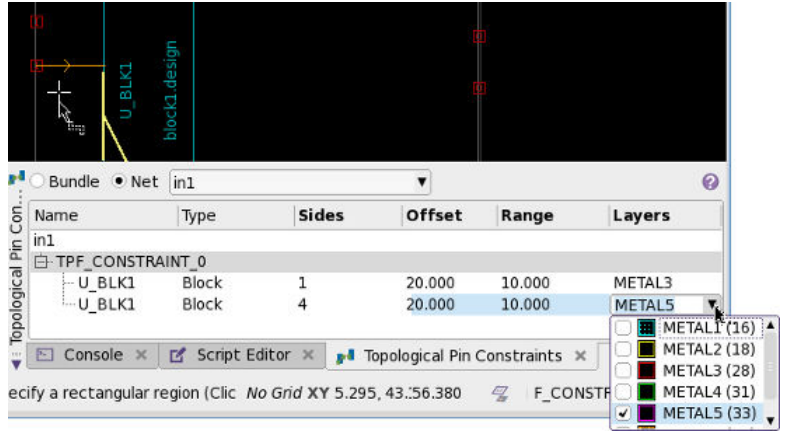
\includegraphics[width=0.92\textwidth]{gui-fig-072.png}
\caption{拓扑管脚约束}
\label{fig:gui-72}
\end{figure}

要为含有多级层次的设计创建拓扑管脚约束，单击 View Settings 面板中的 multiple levels active 框，如下图所示。

\begin{figure}[htbp]
\centering
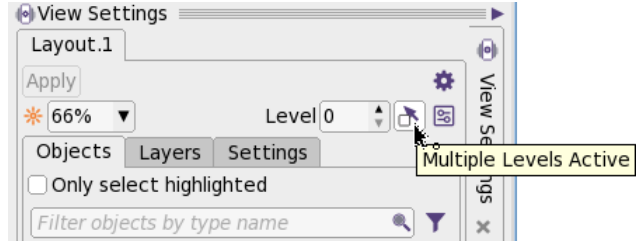
\includegraphics[width=0.92\textwidth]{gui-fig-073.png}
\caption{多级层次处于活动状态}
\label{fig:gui-73}
\end{figure}

\section{使用管脚约束}
\subsection*{Working With Pin Constraints}

使用 Design Assistant 创建、显示和修改单个、成束以及块级管脚约束。

\begin{longtable}{@{}>{\raggedright\arraybackslash}p{0.32\textwidth}>{\raggedright\arraybackslash}p{0.64\textwidth}@{}}
\caption{GUI 支持的管脚约束操作}\label{tab:gui-dp-pin}\\
\toprule
要执行的操作 & 使用此方法 \\
\midrule
\endfirsthead
\caption*{表~\thetable{}（续）：GUI 支持的管脚约束操作}\\
\toprule
要执行的操作 & 使用此方法 \\
\midrule
\endhead
\bottomrule
\endlastfoot
创建管脚约束 &
1. \textbf{Design Assistant > Nets}（或）\textbf{Design Assistant > Pins}\newline
2. 选择线网或束（bundle）（或）选择端口或管脚\newline
3. \textbf{Create > Pin Constraint} \\
\addlinespace
创建块约束 &
在 Design Assistant 中选择 \textbf{Create > Block Pin Constraint} \\
\addlinespace
查看当前设计中的管脚约束与块管脚约束 &
在 Design Assistant 中选择：\newline
\textbullet\ \textbf{View > Pin Constraints of selected}（或）\newline
\textbullet\ \textbf{View > Block Pin Constraints of selected}（或）\newline
\textbullet\ \textbf{View > Pin Constraints}（或）\newline
\textbullet\ \textbf{View > Block Pin Constraints} \\
\addlinespace
显示所选对象上当前已定义的管脚约束 &
在 Design Assistant 中：\newline
1. 选择线网或管脚\newline
2. 右键单击并选择 Get Pin Constraints（或）\textbf{View > Pin Constraints of selected}\newline
管脚约束显示在 PinConstraints 选项卡上。 \\
\addlinespace
显示所选对象上当前已定义的块管脚约束 &
在 Design Assistant 中：\newline
1. 选择块单元（\cmd{is\_soft\_macro == true}）\newline
2. 右键单击并选择 Get Block Pin Constraints（或）\textbf{View > Block Pin Constraints of selected}\newline
管脚约束显示在 BlockPinConstraints 选项卡上。 \\
\addlinespace
删除管脚约束与块管脚约束 &
在 Design Assistant 中选择 \textbf{Edit > Delete Pin Constraints} \\
\addlinespace
选择与管脚约束相关的对象 &
选择管脚约束，再选择 \textbf{Select > Related Objects}，以选择相关的束、线网、管脚或端口 \\
\end{longtable}
